%% Présentation de l'entreprise et de l'endroit où vous vous situez [4-6 pages]

\section{Activité}

La société UINT développe et commercialise des circuits	électroniques fins, souples et autonomes embarqués dans	les cartes à puces. Les docteurs et ingénieurs au service d’UINT déploient leur forte expérience dans la recherche et le développement de l’électronique, de la sécurité des transactions et de la fabrication des cartes à puces, en maîtrisant tous les processus et cycles de vie des produits allant de la conception à la fabrication.\\

UINT a pour ambition d’être le leader mondial sur le marché des cartes à puces ISO dites actives (qui embarquent leur propre source d’énergie). En créant de la valeur ajoutée sur le support carte notamment via l’intégration de ses électroniques flexibles autonomes, UINT permet l’interactivité du porteur avec la carte et vice versa, offrant de nouveaux services disponibles 24h/24h qui vont révolutionner l’utilisation des cartes à puces avec leur environnement.\\

UINT a développé ses propres produits:\\

\begin{itemize}
\item \textit{U-GIFT} est une carte au format bancaire, embarquant une pile, un haut parleur et des diodes. Cette carte peut jouer de la musique et avoir des lumières qui scintillent. Cette carte est destinée au marché de l’affinitaire et de la carte cadeaux. Par exemple, une carte prépayée «joyeux anniversaire» qui peut jouer de la musique en plus de toutes les autres fonctions d’une carte cadeau «traditionnelle».
\item \textit{SPI} (Solution numérique d’impression sécurisée) est une solution logicielle et matérielle permettant de s’assurer que la personne qui imprime un document est la même que celle qui va récupérer les documents sur l’imprimante. Pour simplifier, pour récupérer les documents sur l’imprimante, la personne va devoir s’authentifier via un badge et un code pin.
\item \textit{uSecure} est une carte au format bancaire qui permet de contrôler l’émission d’une trame RF en appuyant sur un bouton. Il s’agit de la première carte RF contrôlée par l’utilisateur.
\end{itemize}


\subsection{Circuits flexibles}
UINT conçoit et développe ses circuits flexibles qui s’insèrent notamment dans des cartes au format bancaire ISO 7810. L’électronique utilisée dans les produits est choisie en fonction de ce critère de flexibilité ainsi que de leur faible consommation.

\begin{figure}[!htbp]
  \centering
    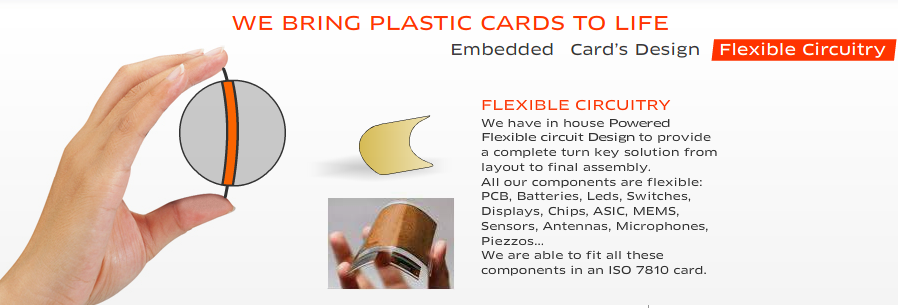
\includegraphics[scale=0.5]{images/flx}
  %\caption{Représentation schématique du cryptogramme}
  %\label{fig:auth}
\end{figure}


\subsection{Sécurité / Identification}

Que ce soit pour l’identification, l’authentification, le contrôle d’accès, le paiement ou tout autre service lié à la sécurité, l’expertise dans le domaine de la sécurité de notre équipe vous garantit une compréhension totale de votre projet.

\begin{figure}[!htbp]
  \centering
    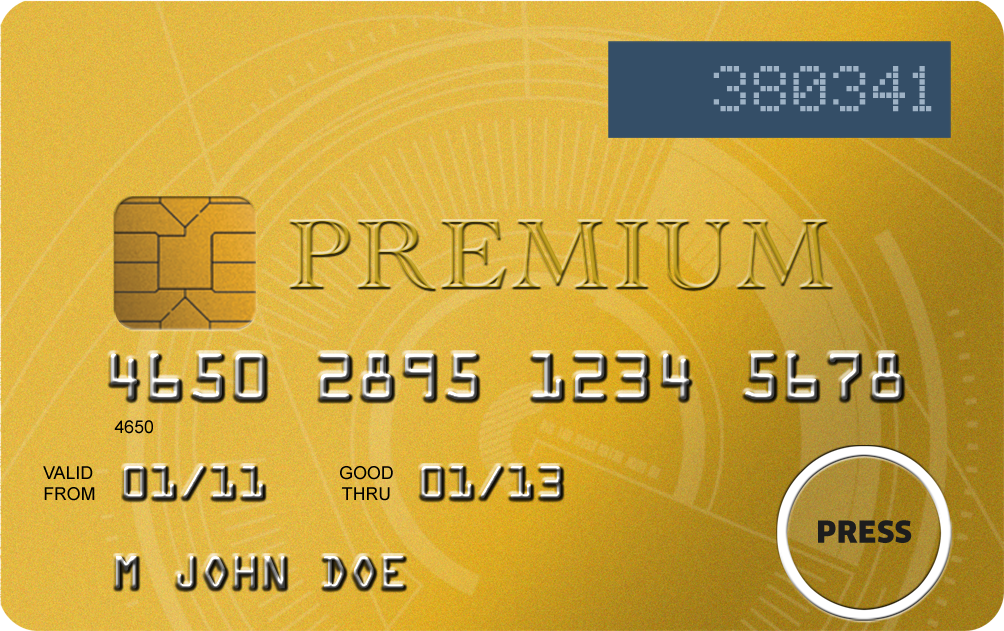
\includegraphics[scale=0.7]{images/pre}
  %\caption{Représentation schématique du cryptogramme}
  %\label{fig:auth}
\end{figure}

Voici quelques exemples de produits phares et voies de développement envisagées:\\

\begin{itemize}
\item Jeu: carte de jeu prépayée
\item Santé: auto contrôle de paramètres physiologiques (pouls, température…)
\item Sécurité: affichage de mot de passe dynamique ; contrôle de l’émission de signature RF, acoustique, biométrie
\item Marketing: carte musicale, à lumière, à écran…
\item Logistique: traçabilité, surveillance de température, capteurs…\\
\end{itemize}

Concernant les modèles de revenus de la société, ces derniers sont variables suivant les projets. Lorsqu’UINT réalise de la R\&D pour ses clients en vue de la fabrication de leurs produits, la société se rémunère sur cette R\&D et bénéficie de royalties ou licences sur les produits. Lorsqu’il s’agit de ses propres produits, par exemple la U-GIFT Card, UINT démarche les grands noms des distributeurs ou émetteurs de cartes cadeaux / fidélité pour mettre la U-GIFT Card dans leur catalogue. Dans ce cas, UINT personnalise la carte (visuel, musique) à la demande du client qui, lui, vendra la carte en «boutique».

\section{Stratégie}

La R\&D est au cœur de l’activité de la société. Sur les 8 salariés, 7 ont une formation de type technique (électronique ou informatique) dont 3 docteurs et 2 ingénieurs. Il est à noter que deux des produits conçus par UINT ont reçu une certification Mastercard.\\ 

Sur le territoire national, UINT n’a aucune concurrence. Au plan international, bien qu’il y ait des sociétés proposant des produits «cartes» avec de l’électronique flexible, aucune ne se positionne comme UINT avec un portfolio de produits aussi variés. Hormis UINT, à notre connaissance, la concurrence ne conçoit et ne produit que des cartes avec un afficheur dans le domaine de la sécurité.\\

Come abordé précédemment, UINT maitrise la conception de circuits flexibles ainsi que la gestion de la faible consommation des composants électroniques.\\

La société UINT a reçu «L’Électron d’Or de la meilleure Start-Up 2010» lors de la cérémonie qui s’est tenue au siège parisien de la FIEEC (Fédération des Industries Électriques, Électroniques et de Communication), le 16 juin 2010. Ce prix est remis par le magazine ÉlectroniqueS et le sponsor RS parmi les 12 lauréats de cette 13ème édition. Les nominés sont des entreprises et des grands groupes nationaux et internationaux (France, Etats-Unis, Allemagne, Royaume-Uni, Norvège, Japon…) repérés par la rédaction du journal à travers l’actualité de leur activité ou de leurs projets. Un jury expert comptant des professionnels du secteur, des consultants et des membres de la rédaction du journal ElectroniqueS est chargé de l’attribution des prix.\\

La société UINT a reçu le prix «de l’innovation à l’internationale 2010» lors du 5ème forum de l’international à Evry le 9 décembre 2010. Ce prix a été décerné par la CGPME 91 et la CCI Essonne.\\

Enfin, la société s’est tournée ces derniers mois vers la Chine en vue d’établir des partenariats technologiques, commerciaux et avec des distributeurs. Depuis le 4 janvier 2011, elle a signé deux contrats avec un partenaire technologique (fabrication de carte) et un distributeur.\\

UINT vient de créer sa propre usine d’hybridation (soudage des composants électroniques au circuit flexible), afin de réduire les coûts de fabrication et augmenter ainsi sa marge. UINT souhaite également agrandir son équipe d’ingénieurs en électronique afin de toujours concevoir de nouveaux produits innovants.

\section{Ressources humaines}

A ce jour, UINT est composée de 8 salariés. UINT fait principalement de la R\&D. Sur les 8 salariés, 7 ont une formation de type technique (électronique ou informatique) dont 2 docteurs et 5 ingénieurs.\\

Ce bilan est antérieur à l’ouverture des Laboratoires sur le site de Limoges et qui doit conduire à l’ouverture d’une vingtaine de postes d’ici fin 2014.

\begin{figure}[!htbp]
  \centering
    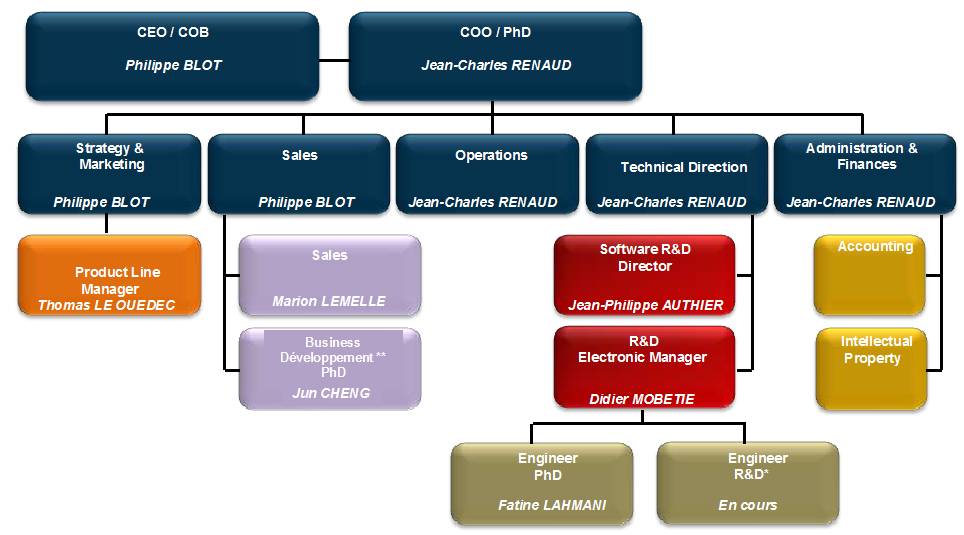
\includegraphics[scale=0.6]{images/rh}
  %\caption{Représentation schématique du cryptogramme}
  %\label{fig:auth}
\end{figure}

\section{Ressources technologiques}

\subsection{Savoir faire et technologies maitrisées}

\begin{itemize}
\item UINT maitrise la conception de circuits fins et flexibles ainsi que la gestion de la faible consommation des composants électroniques.
\item UINT maitrise l'hybridation des composants électroniques sur circuit flexible
\item UINT invente, conçoit, développe et distribue des solutions de cartes multifonctions avec des microprocesseurs sécurisés et autonomes.
\item UINT conçoit et développe des solutions pour authentifier des utilisateurs lors d’échanges sécurisés.
\end{itemize}

\subsection{En termes de protection industrielle, elle possède des brevets}

\begin{itemize}
\item \textit{WO2011067543:} activation et indication d’un champ RF sur un dispositif comprenant une puce
\item \textit{PCT / FR 2010 / 052767:} carte à puce multi-applicatifs avec validation biométrique
\item \textit{FR 2953619:} dispositif électronique (jeton) téléphonique
\end{itemize}

\subsection{Certifications acquises}

A l’heure actuelle, la société UINT ne possède pas de certification, néanmoins deux de ses produits ont reçu une certification Mastercard.


